\section{Methodology}
\begin{figure}[t]
    \centering
    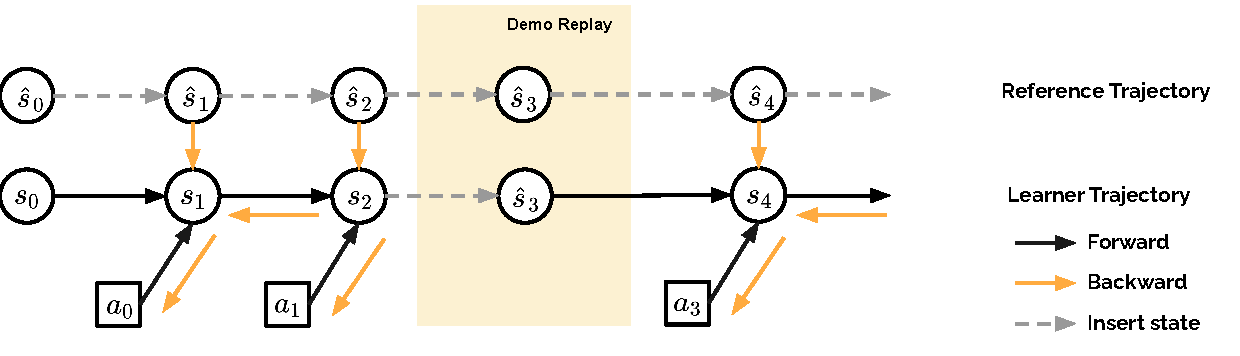
\includegraphics[width=.9\textwidth]{figures/Demo_Replay.pdf}
    \captionof{figure}{Computation graph of DiffMimic. An example of demonstration replay during the third step is demonstrated. The demonstration state in the third step is used to replace the simulated state.}
    \label{fig:computation_graph}
\end{figure}


\subsection{A Motion Mimicking Environment in Differentiable Physics Engine.} 
\textbf{Environment.} We build our environment in Brax~\citep{freeman2021brax}. We design our simulated character following DeepMimic~\citep{peng2018deepmimic}. The humanoid character has 13 links and 34 degrees of freedom.  The character has a weight of 45 kg and a height of 1.62m. Contact is applied to all links with the floor. The environment is accelerated by GPU parallelization. The physics simulator updates at a rate of 480 FPS. The joint limits of the character are relaxed to allow smoother gradient propagation. {We keep the system configurations like friction coefficients consistent with DeepMimic.}

\textbf{State and Action.} States include the position $p$, rotation $q$, linear velocity $\dot{p}$ and angular velocity $\dot{q}$ of all links in the local coordinate. Additionally, following~\citet{peng2018deepmimic}, a phase variable $\phi$ in the range $[0, 1]$ is included in the state to serve as a timestamp. Thus, the state of the environment, $s$, contains the aforementioned information, $s := \{p, q, \dot{p}, \dot{q}, \phi \}$. We follow the common practice and use PD controllers to drive the character. Given the current joint angle $q$, angular velocity $\dot{q}$ and a target angle $\tilde{q}$, the torque on the actuator of the joint will be computed as:
\begin{align}
    \tau = k_p (\tilde{q} - q) + k_d (\tilde{\dot{q}}-\dot{q}),
\end{align}
where $\tilde{\dot{q}}=0$, $k_p$ and $k_d$ are manually-specified gains of the PD controller. We keep $k_p$ and $k_d$ identical to the PD controller used in DeepMimic. A policy network predicts the target angle for the PD controller at each joint. The control policy operates at 30 FPS. 

\subsection{Motion Mimicking with Differentiable Physics}
\algdef{SE}[SUBALG]{Indent}{EndIndent}{}{\algorithmicend\ }%
\algtext*{Indent}
\algtext*{EndIndent}
\begin{wrapfigure}[18]{r}{0.55\textwidth}
\vspace{-23pt}
\begin{minipage}{0.55\textwidth}
\begin{algorithm}[H]
\small
    \caption{DiffMimic}
    \begin{algorithmic}[1]
        \State \textbf{Input:} Optimization Iteration I, Episode Length T, Reference States $\hat{S}=\{\hat{s}_1, \hat{s}_2, \cdots, \hat{s}_t\}$, Error Threshold $\epsilon$.
        \State \textbf{Output:} Optimized policy
        \State Initialize the stochastic policy as \(\pi_\theta\).
        \For{ optimization iteration $i = 1 \cdots I $}
        \State \# Roll out trajectories with Expert Replay
        \State Initialize $s_1 \leftarrow \hat{s}_1$
        \For{ step $t = 1 \cdots T-1 $}
            \begin{equation*}
              s_{t+1} =
                \begin{cases}
                  \mathcal{T}(s_{t}, a_t), \; a_t \sim \pi_{\theta}(a|s_{t}) & \text{if} \; \|s_t-\hat{s}_t\|_2^2 < \epsilon \\
                  \mathcal{T}(\hat{s}_{t}, a_t), \; a_t \sim \pi_{\theta}(a|\hat{s}_{t}) & \text{otherwise.}
                \end{cases}       
            \end{equation*}       
        \EndFor
  
        \State Compute loss
           $ \mathcal{L} =  \sum_{t=1}^T 
            \| s_t - \hat{s}_t \|_2^2$
        
        \State Update the policy \(\pi_\theta\) with analytical gradient \(\bigtriangledown_\theta \mathcal{L}\).

        
        \EndFor
        \State \textbf{Return} the policy \(\pi_\theta\).
\end{algorithmic}
\label{alg:DIL}
\end{algorithm}
\end{minipage}
\end{wrapfigure}
Motion Mimicking is about matching the policy rollout with the reference motion. While it has a straightforward objective, considering human action can be rich and highly flexible, designing a reward to incentivize and guide policy learning is not easy. For example, reward functions that are tailored to guide a policy to learn to walk or learn to backflip can be different and this makes reward engineering difficult. We reveal that the mimicking task can be surprisingly easy when analytical gradients can be obtained through DPS. 

The underlying idea of DiffMimic is to allow the gradient to directly flow back from the distance between reference motion and policy rollout to the policy through an off-the-shelf DPS. We show the computation graph of DiffMimic in Fig.~\ref{fig:computation_graph}. 
Compared with existing RL-based approaches, DiffMimic directly optimizes the policy with supervised state-matching signals and largely eases the reward engineering.
Thanks to the analytical gradient, such an approach has a very high sample efficiency. 
Prior works~\citep{fussell2021supertrack} explored analytic gradients with a learned differentiable world model which describes the dynamics in latent space. However, the learned world model reveals no underlying physics of the system. Consequently, they undermine the effectiveness, generality, and interpretability of the learning with physics-based analytic gradients from DPS, as in DiffMimic. In addition, online learning and inference with learned world models remain computationally expensive when compared with DPS.

We show in detail how to train the policy with DPS. For each iteration, we initialize the state to the first reference state and then roll out to the maximum episode length in a batch of parallel environments. Then we compute the step-wise L2 distance between the rollout trajectory and the reference trajectory in terms of positions and rotations:
\begin{equation}
\begin{gathered}\label{eq:reward}
\tiny
    \mathcal{L} = \sum_{t=1}^T \| s_t - \hat{s}_t\|_2^2, \\
    \| s_t - \hat{s}_t\|_2^2 \triangleq \frac{1}{\|J\|}\sum_{j\in J} w_p(p^j - \hat{p}^j)^2 + w_r(q^j - \hat{q}^j)^2 + w_v(\dot{p}^j - \hat{\dot{p}}^j)^2 + w_a(\dot{q}^j - \hat{\dot{q}}^j)^2, 
\end{gathered}
\end{equation}
where $p^j$ and $\hat{p}^j$ are the global positions of the $j$-th joint from rollout and reference,  $q^j$ and $\hat{q}^j$ are the global rotation of the $j$-th joint from rollout and reference in 6D rotation representation. The weights $w_p$, $w_r$, $w_v$, and $w_a$ only need to be approximately tuned to roughly equalize their magnitudes. Note that we use 6D rotation in loss computation since it is advantageous over quaternions in gradient-based optimization~\citep{zhou2019continuity}. Without loss of generality, we denote the transition function in the dynamic system as $\mathcal{T}$ and the next state of the system can be obtained from the transition function given the current action $a_t$ and character state $s_t$, $s_{t+1} = \mathcal{T}(s_t, a_t)$. In DiffMimic, DPS serves as a transition function $\mathcal{T}$ that is fully differentiable. Thus, from the loss function, we can directly derive the gradient with respect to both the current action $a_t$ and state $s_t$
\begin{equation}
\small
    \frac{\partial \mathcal{L}}{\partial a_t} = \left(\frac{\partial \mathcal{L}}{ \partial\mathcal{T} (s_t, a_t)}\right)\left(\frac{\partial \mathcal{T}(s_t, a_t)}{\partial a_t}\right),\quad \frac{\partial \mathcal{L}}{\partial s_t} = \left(\frac{\partial \mathcal{L}}{ \partial\mathcal{T} (s_t, a_t)}\right)\left(\frac{\partial \mathcal{T}(s_t, a_t)}{\partial s_t}\right).
\end{equation}
By doing this recursively, the gradient can be propagated through the whole trajectory. 











\begin{figure}[t!]
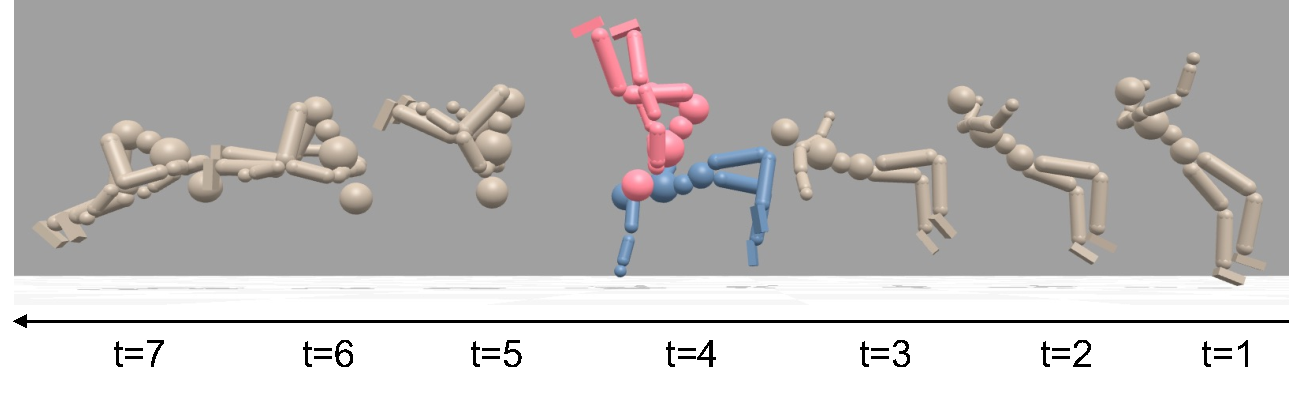
\includegraphics[width=0.8\textwidth]{figures/qp/expert_replay5.pdf}
\centering
\caption{Illustration of \ourmethod{}, which happens when t=4 where the character is about to fall. The rollout state (in blue) is replaced by the reference state (in red) for the next step.}
\end{figure}
\subsection{Demonstration Replay}
Although mimicking with DPS results in a succinct learning framework, there are three well-known challenges in policy learning with DPS: 1) Exploding/vanishing gradients with the long horizon; 2) Local minima may cause gradient-based optimization methods to stall; 3) Noisy or wrong gradients.

We observe that the high non-convexity in the motion mimicking task poses severe challenges to analytical gradient-based optimization. Due to the local nature of the analytical gradients, the policy can be easily stuck at suboptimal points. As shown \autoref{fig:vis_ablation}, when trying to mimic the \textit{Backflip} skill, the character learns to use arms to support itself instead of exploring a more dynamic jumping move. 
In practical implementations, dividing the whole trajectory into smaller sub-trajectories for truncated Back-Propagation-Through-Time (BPTT) further exacerbates the issue.
As shown in \autoref{tab:ablation} (a)-(b), a 10-step gradient truncation leads the policy to a less favorable local optimal.

Teacher forcing~\citep{williams1989learning} is a common remedy to escape the local minimum in gradient-based sequential modeling. Teacher forcing randomly replace the states in rollout by the reference states.
Given a teacher forcing ratio $\gamma$:
\begin{equation}
  s_{t+1} =
    \begin{cases}
      \mathcal{T}(s_{t}, a_t), \; a_t \sim \pi_{\theta}(a|s_{t}) & \text{if} \; b=0, b\sim \textrm{Bernoulli}(\gamma)\\
      \mathcal{T}(\hat{s}_{t}, a_t), \; a_t \sim \pi_{\theta}(a|\hat{s}_{t}) & \text{otherwise.}
    \end{cases}       
\end{equation}   


However, although the mechanism leads to a better global optimal overall, it does not guarantee the character to faithfully mimic the reference motion in each frame. As shown in \autoref{fig:vis_ablation}, although the character's overall trajectory matches the reference, several frames suffer from awkward poses. \autoref{fig:frame_loss} shows that a few frames have significantly larger pose errors than other frames.

We propose demonstration-guided exploration to mitigate these challenges in DPS for policy learning to help exploration and encourage faithfully mimicking at the same time. The main idea of demonstration-guided exploration is to replace states in the policy rollout with the corresponding demonstration states when the states are too far away from the reference. For a threshold $\epsilon$:
\begin{equation}
  s_{t+1} =
    \begin{cases}
      \mathcal{T}(s_{t}, a_t), \; a_t \sim \pi_{\theta}(a|s_{t}) & \text{if} \; \|s_t-\hat{s}_t\|_2^2 < \epsilon \\
      \mathcal{T}(\hat{s}_{t}, a_t), \; a_t \sim \pi_{\theta}(a|\hat{s}_{t}) & \text{otherwise.}
    \end{cases}       
\end{equation}   
Since the criterion for choosing which states to replace is based on the performance of the current rollout, the replacing frequency dynamic adjusts itself during the model training.




